\section{Running Demo}
\label{sec:impl:mockup}

The Phase~One demo runs end-to-end against the warehouse and shows the
visual contract of Section~\ref{sec:solution:interaction} at its three
levels: the overview hub, the inside of a theme, and the scrolling
story. Every figure below is a screen capture of the running
application, taken from the live demo at a 1600-pixel browser width.

\noindent\textbf{Overview hub.} The hub is the landing page. It lays the
six themes out as a long editorial scroll, alternating image-left and
image-right, each with a one-line finding, three supporting numbers, and
a link into the story where one exists. A strip of six headline numbers
sits under the hero, read live from the warehouse on each request.

\begin{figure}[!htbp]
\centering
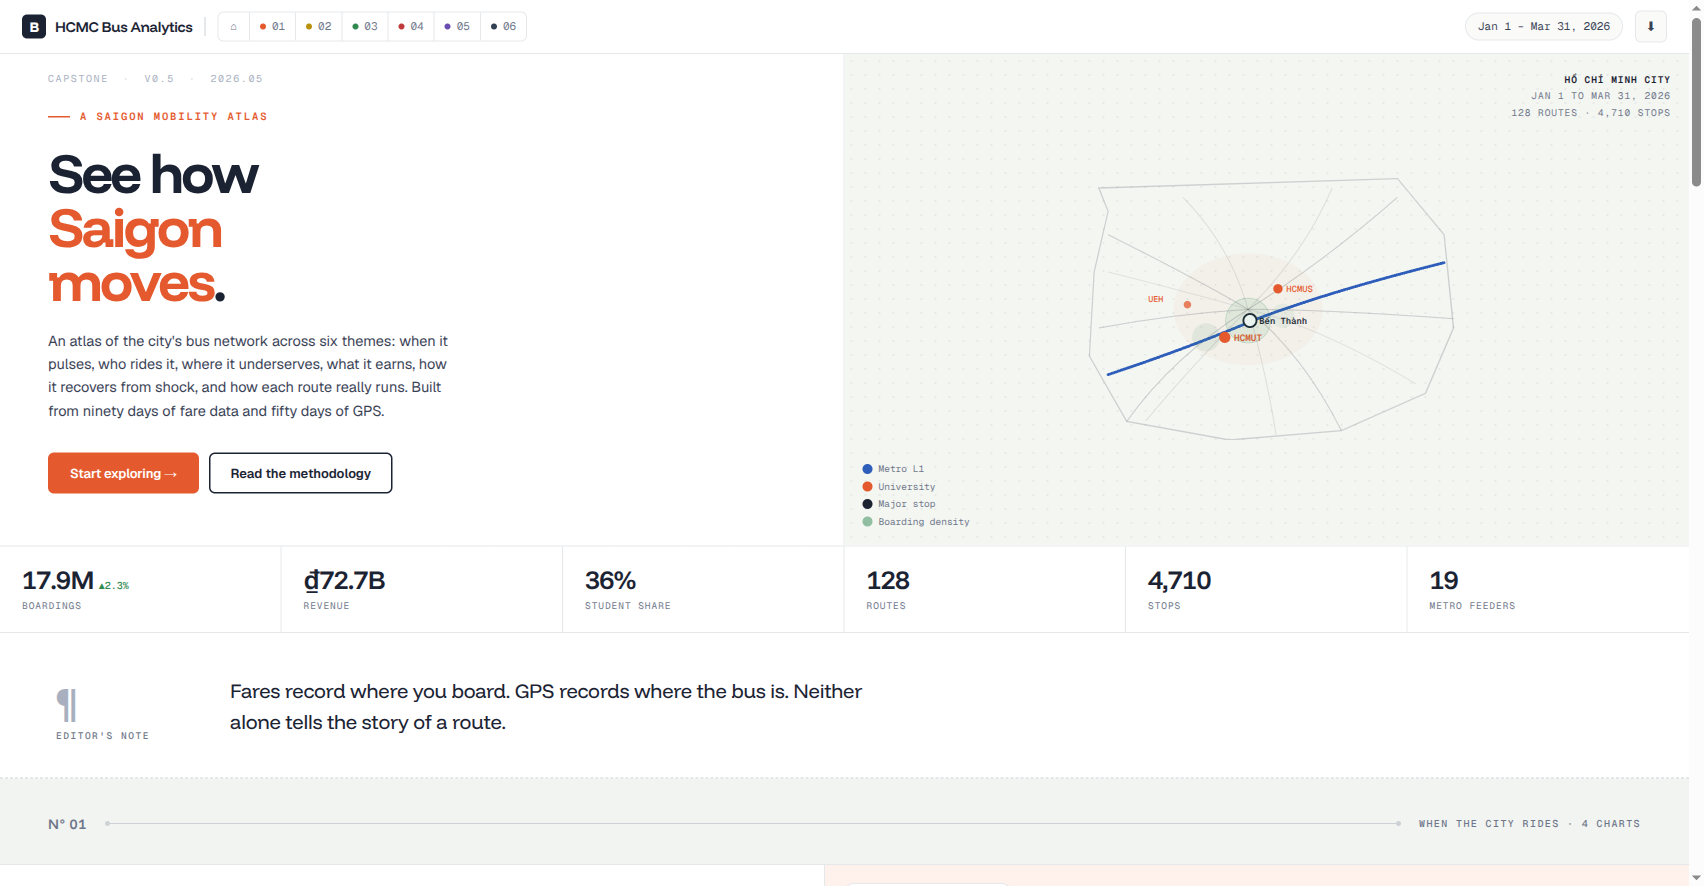
\includegraphics[width=\linewidth,height=0.46\textheight,keepaspectratio]{images/screenshots/demo_hub.png}
\caption{The overview hub with live network KPIs.}
\label{fig:impl:demo:hub}
\end{figure}

\noindent\textbf{Inside a theme.} A theme keeps the chart picker on a
left rail, the finding and its supporting line in the chart header, the
chart filling the centre, and a short source line beneath. The
school-aware demand theme opens on a bubble chart of the universities,
then a treemap of how their students split across routes.

\begin{figure}[!htbp]
\centering
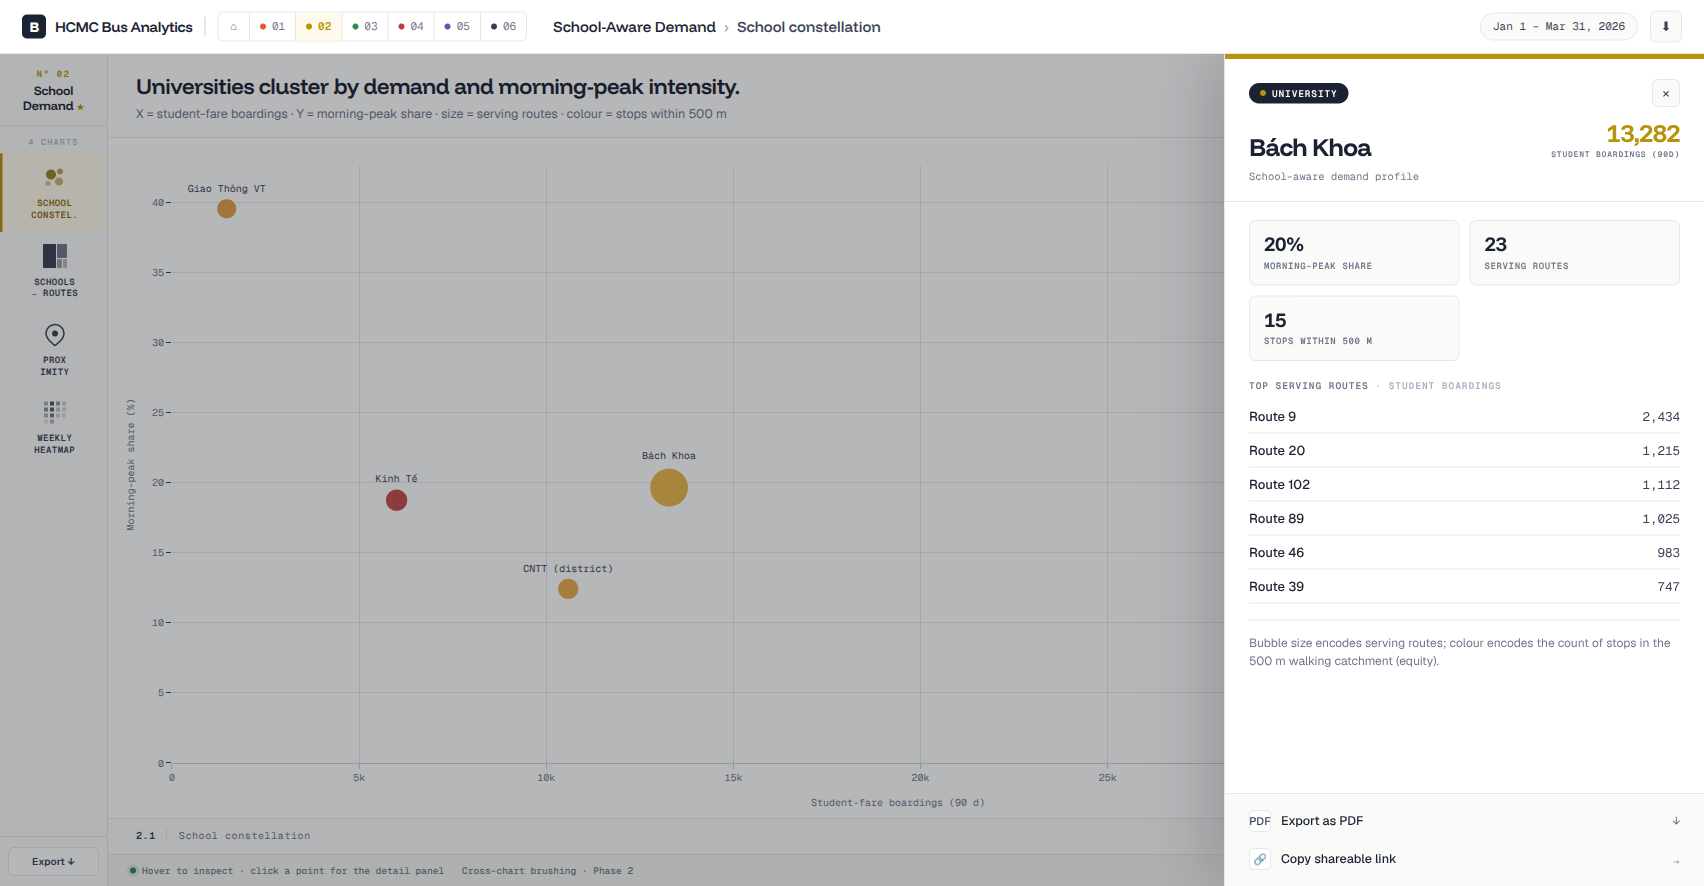
\includegraphics[width=\linewidth]{images/screenshots/demo_card_school_constellation.png}
\caption{School-aware demand theme: university constellation with entity panel open.}
\label{fig:impl:demo:constellation}
\end{figure}

\begin{figure}[!htbp]
\centering
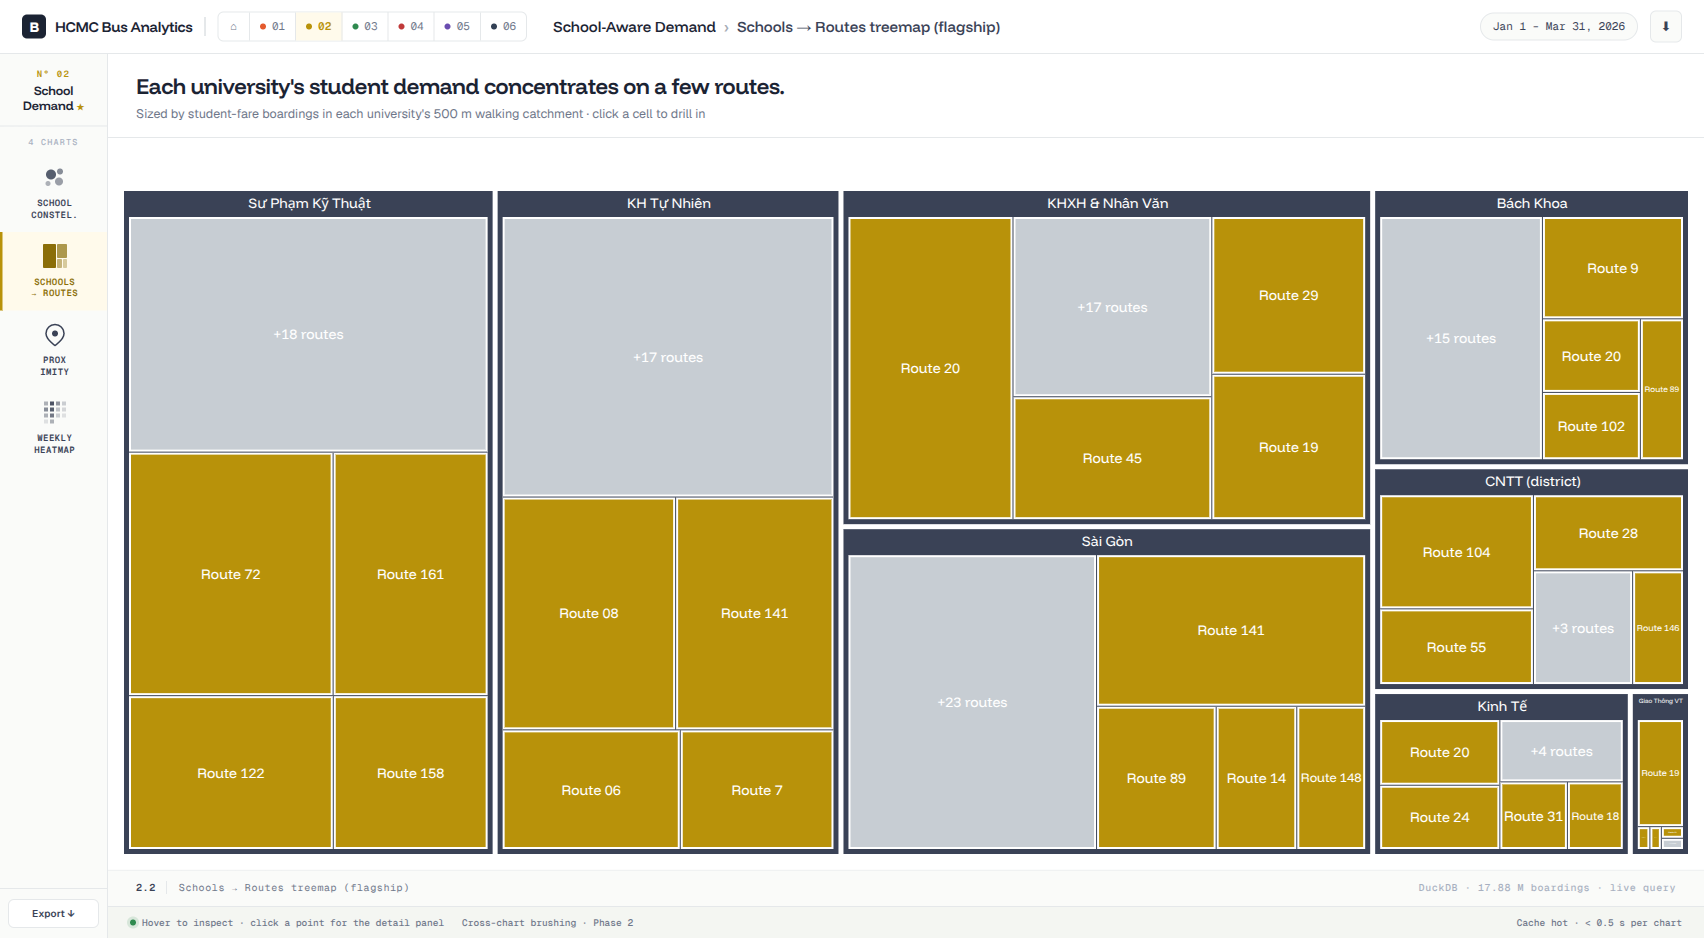
\includegraphics[width=\linewidth]{images/screenshots/demo_card_school_treemap.png}
\caption{School-to-route treemap: student demand by route per university.}
\label{fig:impl:demo:treemap}
\end{figure}

\noindent\textbf{Spatial and network-health themes.} The spatial theme
opens on a boarding-density map and also carries a reach map from a
chosen hub. The network-health theme opens on the reliability view and
carries the daily pulse with the T\^et drop marked.

\begin{figure}[!htbp]
\centering
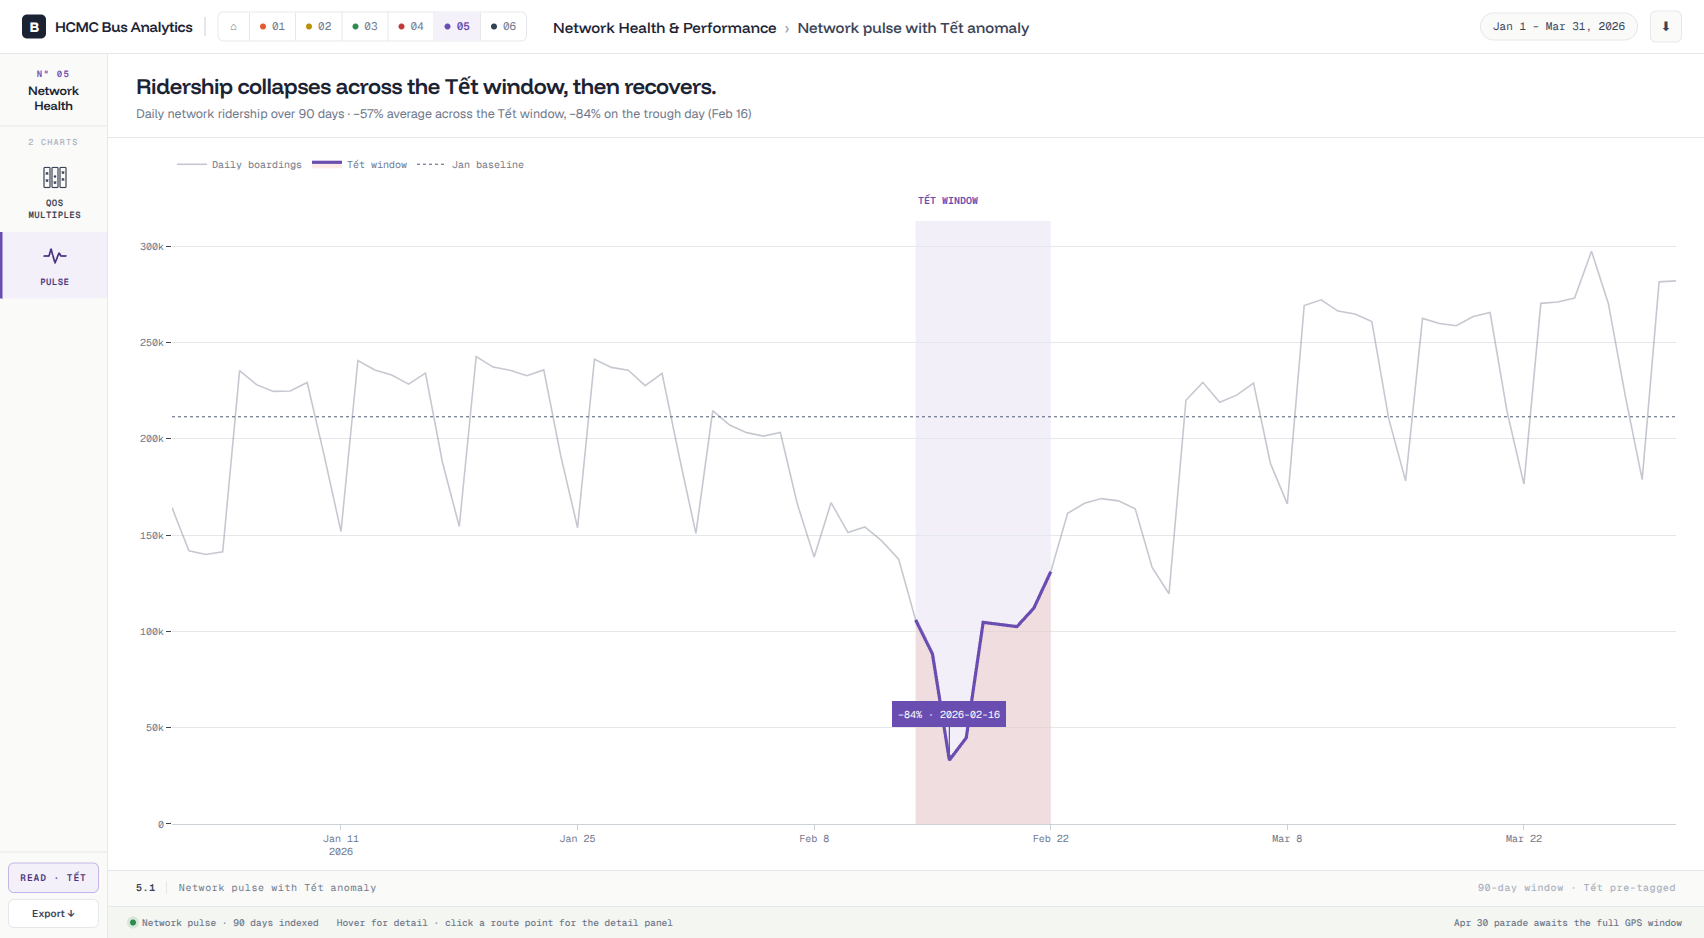
\includegraphics[width=\linewidth]{images/screenshots/demo_card_health_pulse.png}
\caption{Daily network pulse with the T\^et window shaded and trough day flagged.}
\label{fig:impl:demo:pulse}
\end{figure}

\begin{figure}[!htbp]
\centering
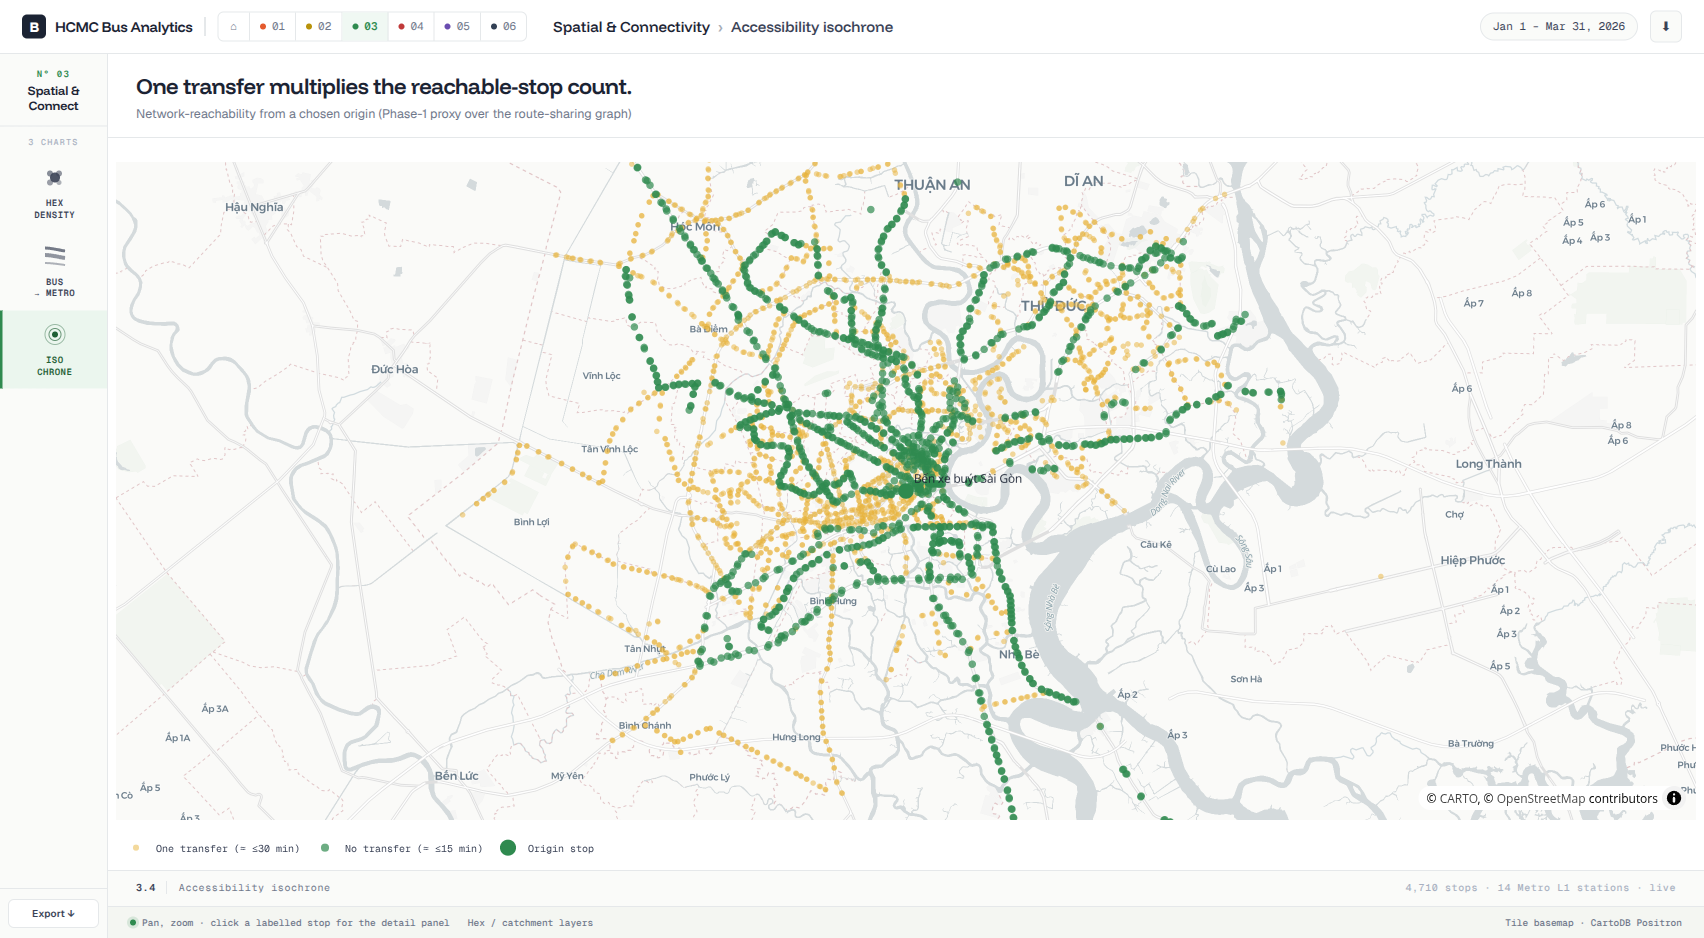
\includegraphics[width=\linewidth]{images/screenshots/demo_card_spatial_isochrone.png}
\caption{Network reach map: direct stops and one-transfer stops from a central hub.}
\label{fig:impl:demo:isochrone}
\end{figure}

\begin{figure}[!htbp]
\centering
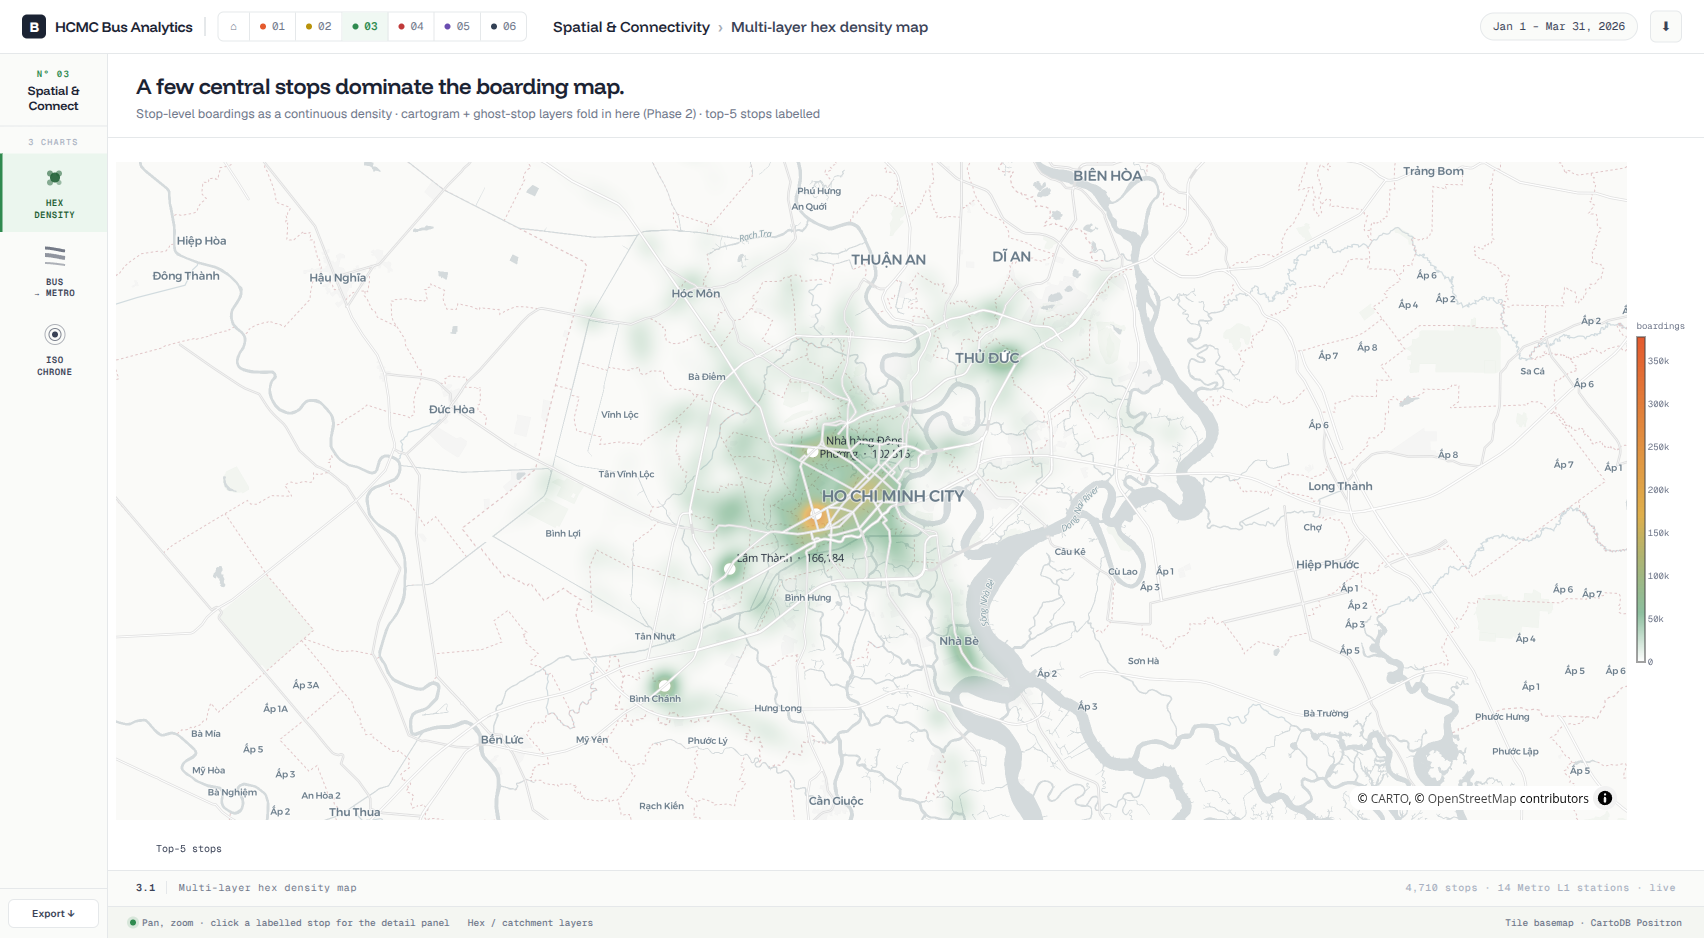
\includegraphics[width=\linewidth]{images/screenshots/demo_card_spatial_hex.png}
\caption{Boarding density map with the five busiest stops labelled.}
\label{fig:impl:demo:hex}
\end{figure}

\begin{figure}[!htbp]
\centering
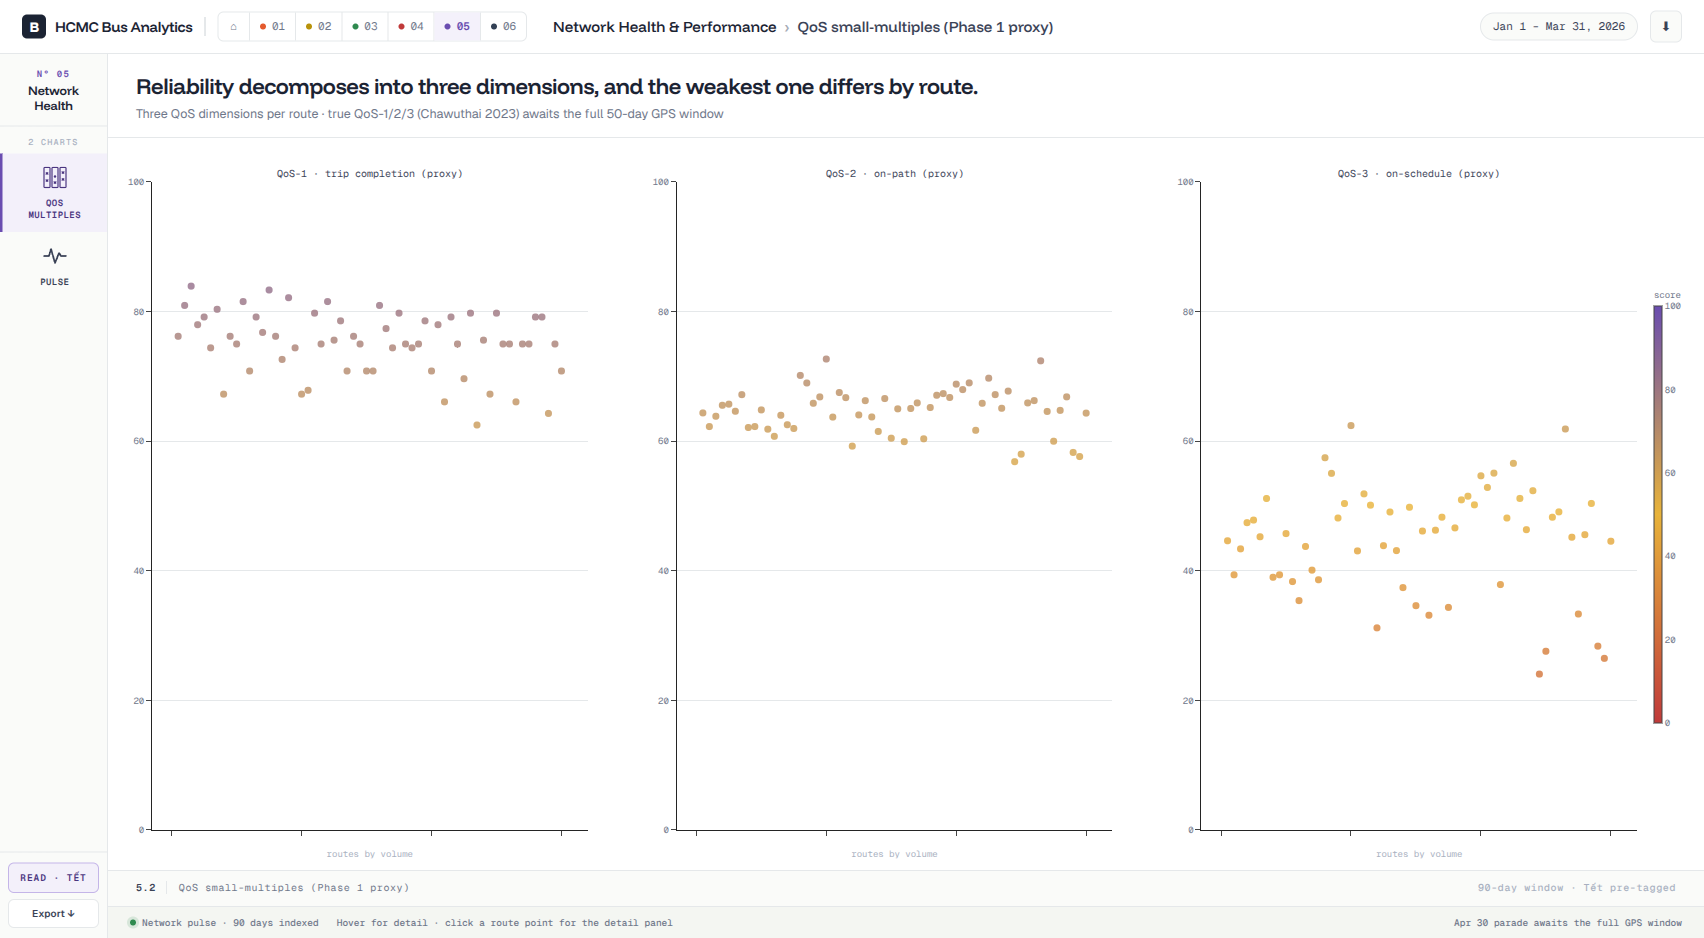
\includegraphics[width=\linewidth]{images/screenshots/demo_card_health_qos.png}
\caption{Route reliability scorecard, three QoS measures.}
\label{fig:impl:demo:qos}
\end{figure}

\noindent\textbf{Clicking through.} A click is the one link between a
chart and the rest of the screen: clicking any point, bubble, or stop
slides in a panel on the right with that item's name, its headline
number, a few supporting figures, and a short list of related routes,
all read from the warehouse. Figure~\ref{fig:impl:demo:constellation}
shows that panel open for a university, listing the routes that carry its
students.

\noindent\textbf{The story.} The T\^et story (``\textit{Nine days
without a network}'') turns the shock into a guided read. The whole
story is one full-screen dark stage that advances as the reader scrolls,
like a slide deck: the writing moves up and out at the top while the
chart underneath changes in place. It opens on a single headline number,
walks through the drop day by day, and closes with a short recap.

\begin{figure}[!htbp]
\centering
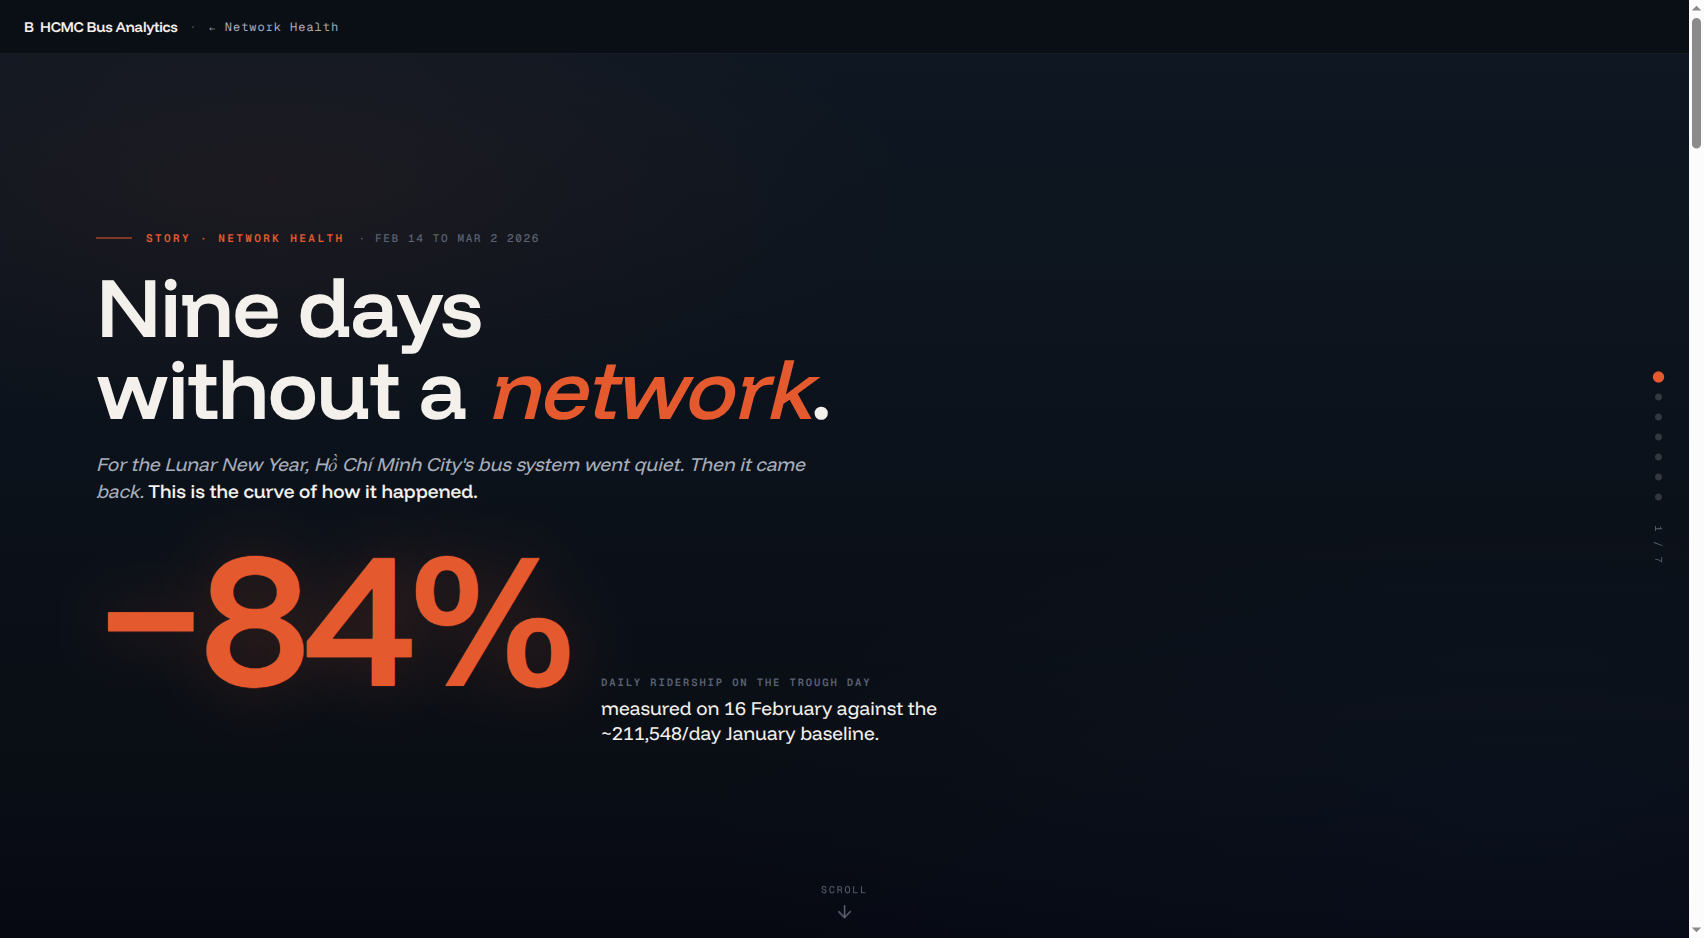
\includegraphics[width=\linewidth]{images/screenshots/demo_story_tet.png}
\caption{T\^et story: opening hero frame.}
\label{fig:impl:demo:story}
\end{figure}

\begin{figure}[!htbp]
\centering
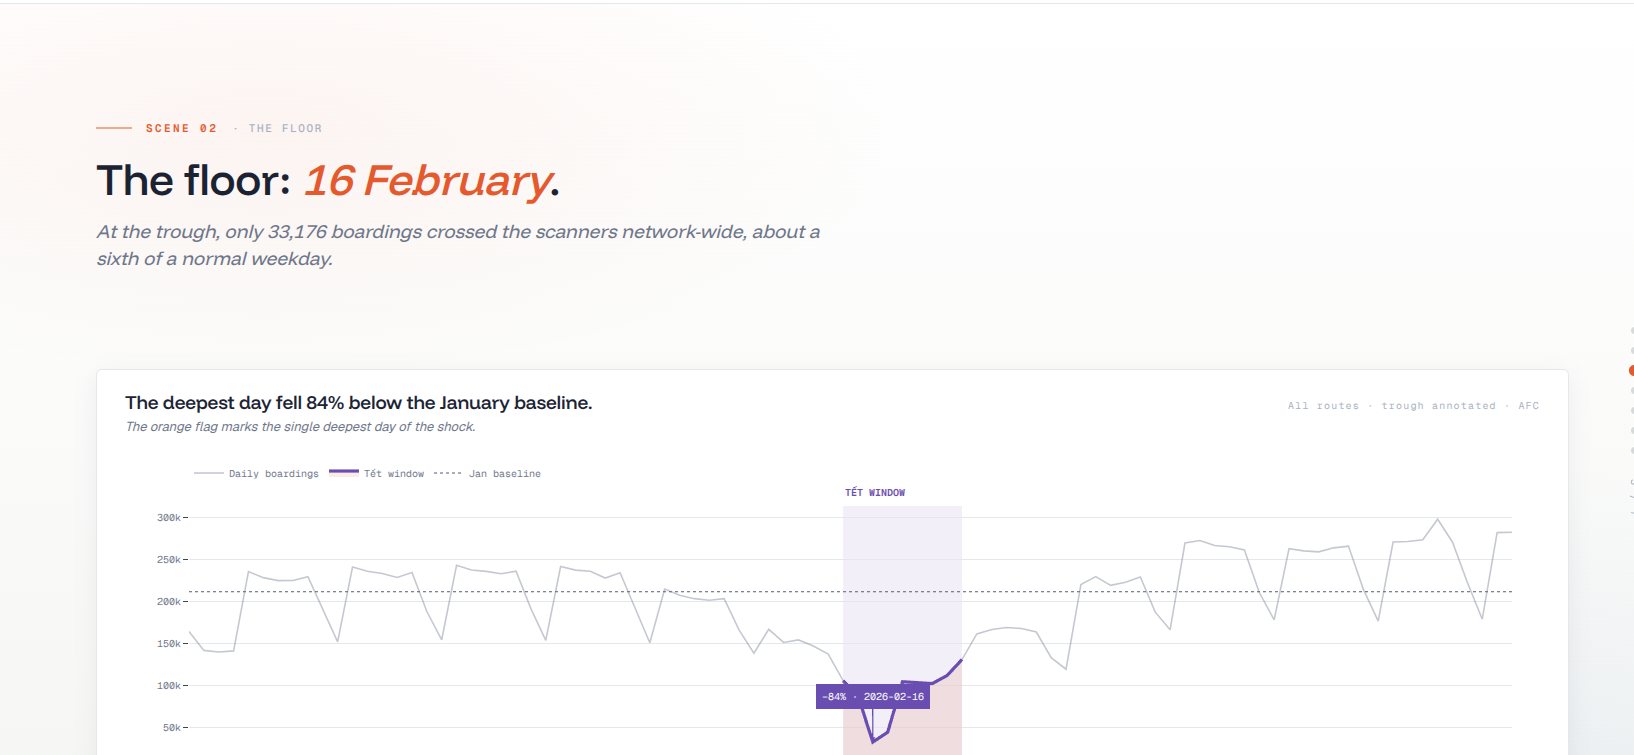
\includegraphics[width=\linewidth]{images/screenshots/demo_story_tet_drop.png}
\caption{T\^et story: drop step with shaded window.}
\label{fig:impl:demo:story:drop}
\end{figure}

\begin{figure}[!htbp]
\centering
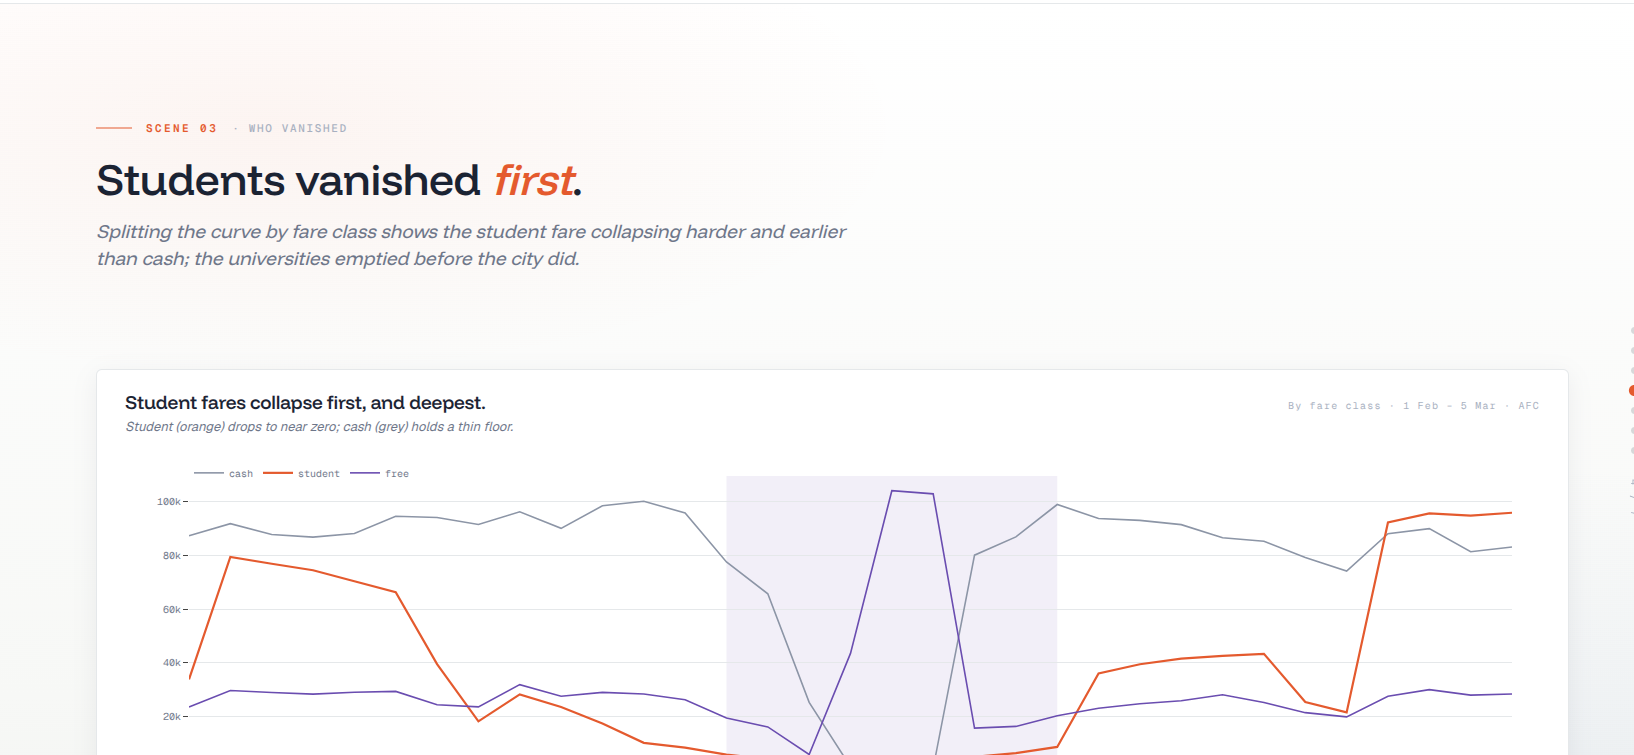
\includegraphics[width=\linewidth]{images/screenshots/demo_story_tet_fareclass.png}
\caption{T\^et story: fare-class breakdown step.}
\label{fig:impl:demo:story:fareclass}
\end{figure}

\begin{figure}[!htbp]
\centering
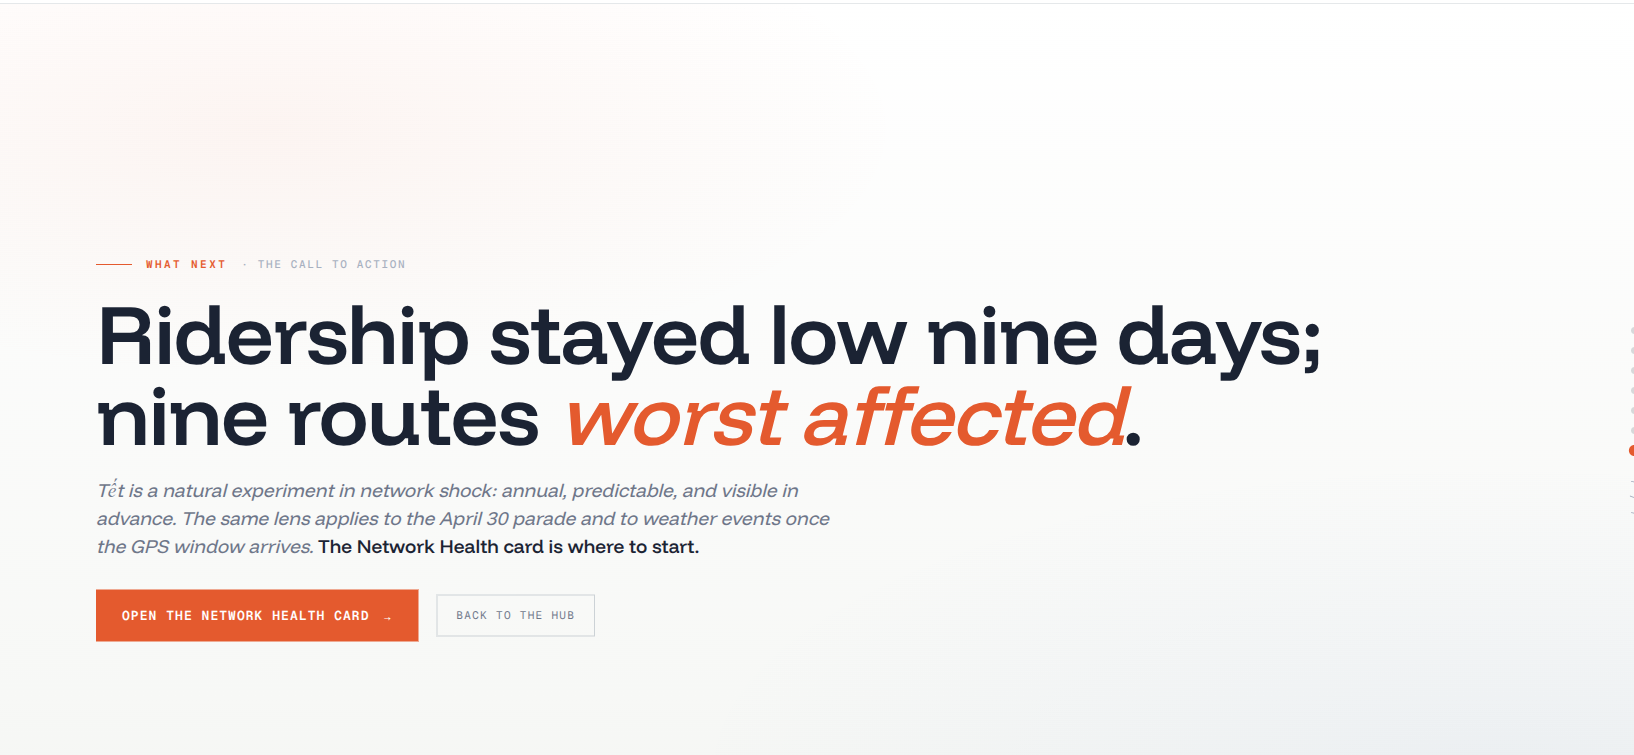
\includegraphics[width=\linewidth]{images/screenshots/demo_story_tet_bongo.png}
\caption{T\^et story: closing recap.}
\label{fig:impl:demo:story:bongo}
\end{figure}

Together the figures show the three ways the tool is used: pick a chart
on the rail and the centre and the page address both update without the
rest of the page moving; click an item and its detail panel opens; or
read a theme as a scrolling story. The writing rules from
Section~\ref{sec:solution:interaction} hold across every chart: the
title states the finding, the line under it gives the context, bars
start at zero, bright colour is saved for the one thing the chart points
at, and each chart reads in a few seconds. The detail panel works today;
the one piece still left for Phase~Two is keeping a selection
highlighted across several charts at once, noted in the self-check of
Section~\ref{sec:impl:eval}.
